% arara: lualatex
% arara: lualatex
% Typeset using lualatex

\documentclass[a4paper,10pt]{article}
\usepackage[utf8]{luainputenc}
\usepackage[pdfborder={0 0 0}]{hyperref}

\usepackage[english]{babel}

\usepackage{fouriernc}
\usepackage{tgpagella}
\usepackage{xcolor}
\usepackage[activate=true]{microtype}
\usepackage{amssymb}
\usepackage{fontspec}
\usepackage{titling}
\usepackage{titlesec}

\usepackage{calc}
\usepackage{multicol}
\usepackage{array}
\usepackage{enumitem}
\usepackage{tikz}
\usepackage{pgfplots}
\usepackage{siunitx}
\usepackage{colortbl}
\usepackage[a4paper,margin=2cm,top=1cm]{geometry}

\setmainfont[Numbers=OldStyle]{TeX Gyre Pagella}

\definecolor{plhome}{HTML}{CCEEFF}
\definecolor{silver}{HTML}{DDDDDD}

\pagestyle{empty}

\parskip=1ex
\parindent=0pt

\setlist[enumerate,1]{start=0}

\newcommand\plpage{
    \newpage
    \begin{tikzpicture}[remember picture,overlay]
        \node[opacity=0.1,below left,xshift=1cm,yshift=1cm] at (current page.north east) {\includegraphics[width=12cm]{../logo}};
    \end{tikzpicture}
}

\newcommand\answerspace{\\\rule[0cm]{0pt}{1cm}}

\newcommand\True{\texttt{True}}
\newcommand\False{\texttt{False}}

\newcommand\startsection[1]{
     \vspace{0.2ex}
    \hrule
    {\fontspec{Oxygen} \tiny
     \vspace{-1ex}
     \emph{#1}
     \vspace{-1.5em}
    }
}

\newfontfamily\headingfont[]{Bree Serif}
\titleformat*{\section}{\LARGE\headingfont}

\begin{document}

\plpage

\section*{Blinking LED with MicroPython on ESP32}

\begin{enumerate}
\item Set up your environment. Ask booth staff for the proper handout.

\end{enumerate}

\startsection{Controlling the LED.}

\begin{enumerate}[resume]

\item MicroPython allows you to read or control several pins.
      To do that, you need to import the \texttt{Pin} class
      with \texttt{from machine import Pin}.

\item A pin can serve as a binary data input or output.
      On hardware side, imagine there either is electricity or there isn't.
      On software side you can either read \emph{zero} or \emph{one} from the pin
      or write that information into it.
      To write the information you initialize a \texttt{Pin} object with
      \texttt{Pin(number, Pin.OUT)}.
      The integrated \emph{Light Emitting Diode} (LED) is available on pin number 2.
      Save a variable with the pin, such as \texttt{led = Pin(2, Pin.OUT)}

\item Set 1 to turn the light on: \texttt{led.value(1)}

\item Set 0 to turn the light off: \texttt{led.value(0)}

\end{enumerate}

\startsection{Blinking the LED with a button.}

\begin{enumerate}[resume]

\item You'll create a program that turns the LED on when the user is holding a button.
      To read the value of the \emph{BOOT} button, create an input pin number 0.

      \texttt{~~~~button = Pin(0, Pin.IN)}

\item Read the value with \texttt{button.value()}. What is it?

\item Read the value while holding the \emph{BOOT} button. What is it?

\item Using an infinite loop, make the LED shine if and only if you hold the button.

\item Change the program so one press of the button switches the light.
      Is there a problem? How do you check for one press?

\end{enumerate}

\startsection{Blinking the LED with sleep.}

\begin{enumerate}[resume]

\item Let's blink the LED. You can use the \texttt{sleep} function form the \texttt{time} module.
      Make the LED blink 10 times with a half second interval.

\end{enumerate}

\startsection{Blinking with Pulse Width Modulation.}

\begin{enumerate}[resume]

\item Make the LED blink really fast.
      On for $\frac{1}{1000}$ of a second, off for $\frac{2}{1000}$ of a second.
      What happens? What if you swap the numbers?
      This is how light intensity is controlled: with fast blinking.

\item Fast blinking with sleep is not very effective.
      You can use the integrated hardware \emph{Pulse Width Modulation} (PWM).
      Imagine a rectangular wave as drown here:

      % https://tex.stackexchange.com/a/113050/51382
      \begin{center}
      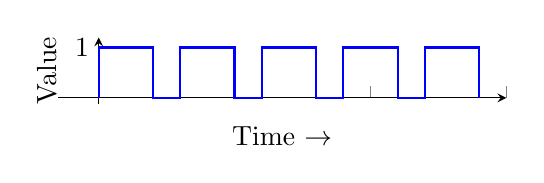
\begin{tikzpicture}
      \begin{axis}[
      width=.6\textwidth,
      height=.2\textwidth,
      x axis line style={-stealth},
      y axis line style={-stealth},
      ymax = 1.2,xmax=15,
      axis lines*=center,
      ytick={0,1},
      xticklabels={},
      xlabel={Time $\rightarrow$},
      ylabel={Value},
      xlabel near ticks,
      ylabel near ticks]
      \addplot+[thick,mark=none,const plot]
      coordinates
      {(0,0) (0,1) (2,0) (3,1) (5,0) (6,1) (8,0) (9,1) (11,0) (12,1) (14,0)};
      \end{axis}
      \end{tikzpicture}
      \end{center}

      A PWM will change the value of a pin from 0 to 1 and back in a periodic interval.
      The \texttt{PWM} class from the \texttt{machine} module takes 3 arguments:
      a pin, frequency and duty.

      \texttt{~~~~pwm = PWM(led, freq=50, duty=512)}

      Frequency determines how fast the LED will blink.
      Duty determines the proportion of time where the LED is on, where 0 means never and 1023 means always.
      When experimenting, mind the fact that humans don't perceive light intensity linearly.

      With PWM running, you can do other things in Python -- it is not blocking.
      To change a PWM's frequency or duty, use the \texttt{pwm.freq(...)} or \texttt{pwm.duty(...)} methods.
      To stop a PWM, use the \texttt{pwm.deinit()} method.

\end{enumerate}

\end{document}
